 \section{PGraph relabeling systems with priorities (PGLS)}
    Graph relabeling system with Priority is a graph relabeling system with a set of graph relabeling rules organized under a strict partial order. The priority mechanism ensures that certain rules are applied on certain area only when no higher-priority rules are applicable. This restriction depends on the order on the rules, and thus cannot be achieved by restricting the matching mechanism. In this section, we proposed to restrict the definition of a relabeling system via a rewriting framework.

 

    \begin{definition}
    \end{definition}
    
    \begin{definition}[Graph relabeling system with priority relation on rules]
      \label{def:pgls_framework}
    
      Let $\mathcal{R}$ be a set of graph relabeling rules and $<$ a strict partial order on $\mathcal{R}$.
    
      We defined a rewriting framework, denoted $\mathfrak{pgls}(\mathcal{R},<)$, as follows: for all $\rho \in \mathcal{R}$,
      $\mathfrak{pgls}(\mathcal{R},<)(\rho)$ is the classe of all witnesses of rewriting steps
      $\left(  m_\rho, m'_\rho \right)$ using the rule $\rho$
      such that there does not exist 
      a rule $\sigma \in \mathcal{R}$ with $\sigma > \rho$ and a witness of a rewriting step
      $\left(  m_\sigma, m'_\sigma \right)$ using the rule $\sigma$ such that 
      $\operatorname{Im}(m_\rho) \cap \operatorname{Im}(m_\sigma) \neq \emptyset$.
 
      The structure $(\mathbf{Graph},\mathcal{R},M,W,\mathfrak{M},\mathfrak{W},\mathfrak{I}, \mathfrak{pgls}(\mathcal{R},<))$, where $M, \mathfrak{M}, W , \mathfrak{W}, \mathfrak{I}$ are the match, match mechanism, witnesses, witness function and interpretation functions introduced in Definition~\ref{def:gls:rewriting}, defines a rewriting system, called \textbf{graph relabeling system with priority relation on rules (PGLS)}. 

    \end{definition}
     
     
    \todo{example: ref,  explanation}
    \begin{example}
      \label{example:pgrs_spanning_tree}
      Consider the GRS \(\mathcal{R}= \{r_1,r_2\}\) with \(\Sigma = \{N, A, 0, 1\}\) and \(r_1 > r_2\). The rules \(r_1\) and \(r_2\) are depicted below:
      
      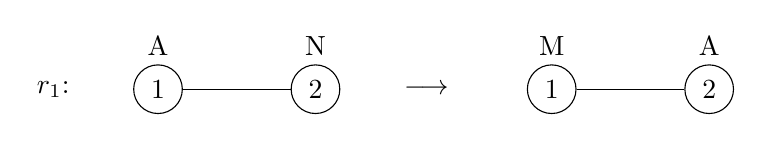
\begin{tikzpicture}
      \draw (-1,0) node[left] {$r_1$:};
      
      \node[draw,circle] (x_1) at (0,0) {$1$};
      \draw (0,0.3) node[above]{A};
      \node[draw,circle, minimum size = 1pt] (x_2) at (2,0) {$2$};
      \draw (2,0.3) node[above]{N};
      \draw[-] (x_1) -- (x_2);
      
      \draw (3,0) node[right] {$\longrightarrow$};
      
      \node[draw,circle] (x3) at (5,0) {$1$};
      \draw (5,0.3) node[above]{M};
      \node[draw,circle, minimum size = 1pt] (x4) at (7,0) {$2$};
      \draw (7,0.3) node[above]{A};
      \draw[-] (x3) -- (x4);
      \end{tikzpicture}
      
      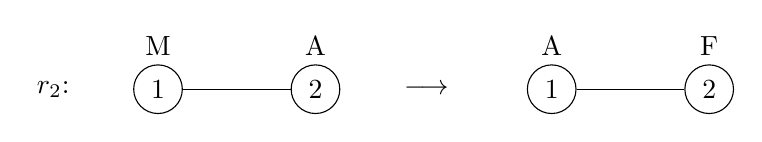
\begin{tikzpicture}
      \draw (-1,0) node[left] {$r_2$:};
      
      \node[draw,circle] (x_1) at (0,0) {$1$};
      \draw (0,0.3) node[above]{M};
      \node[draw,circle, minimum size = 1pt] (x_2) at (2,0) {$2$};
      \draw (2,0.3) node[above]{A};
      \draw[-] (x_1) -- (x_2);
      
      \draw (3,0) node[right] {$\longrightarrow$};
      
      \node[draw,circle] (x3) at (5,0) {$1$};
      \draw (5,0.3) node[above]{A};
      \node[draw,circle, minimum size = 1pt] (x4) at (7,0) {$2$};
      \draw (7,0.3) node[above]{F};
      \draw[-] (x3) -- (x4);
      \end{tikzpicture}
    \end{example}
     
\begin{example}
  to do example

  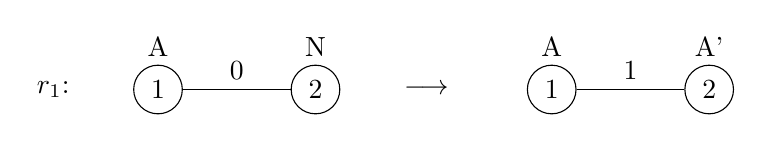
\begin{tikzpicture}
		\draw (-1,0) node[left] {$r_1$:};
		\draw (1,0) node[above] {0};
		
		\node[draw,circle] (x_1) at (0,0) {$1$} ;
		\draw (0,0.3) node[above]{A};
		\node[draw,circle, minimum size = 1pt] (x_2) at (2,0) {$2$};
		\draw (2,0.3) node[above]{N};
		\draw[-] (x_1) -- (x_2);
		
		\draw (3,0) node[right] {$\longrightarrow$};
		\draw (6,0) node[above] {1};
		
		\node[draw,circle] (x3) at (5,0) {$1$} ;
		\draw (5,0.3) node[above]{A};
		\node[draw,circle, minimum size = 1pt] (x4) at (7,0) {$2$};
		\draw (7,0.3) node[above]{A'};
		\draw[-] (x3) -- (x4);
	\end{tikzpicture}
	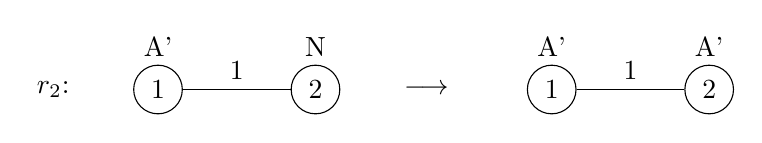
\begin{tikzpicture}
		\draw (-1,0) node[left] {$r_2$:};
		\draw (1,0) node[above] {1};
		
		\node[draw,circle] (x_1) at (0,0) {$1$} ;
		\draw (0,0.3) node[above]{A'};
		\node[draw,circle, minimum size = 1pt] (x_2) at (2,0) {$2$};
		\draw (2,0.3) node[above]{N};
		\draw[-] (x_1) -- (x_2);
		
		\draw (3,0) node[right] {$\longrightarrow$};
		\draw (6,0) node[above] {1};
		
		\node[draw,circle] (x3) at (5,0) {$1$} ;
		\draw (5,0.3) node[above]{A'};
		\node[draw,circle, minimum size = 1pt] (x4) at (7,0) {$2$};
		\draw (7,0.3) node[above]{A'};
		\draw[-] (x3) -- (x4);
	\end{tikzpicture}\\
	avec $r_2 > r_1$.

%1
  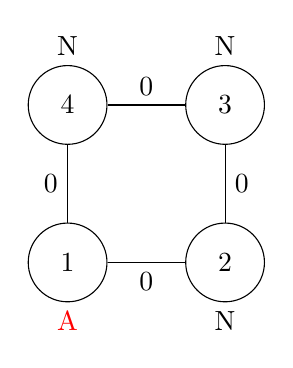
\begin{tikzpicture}
		\node[draw, circle, minimum size = 1 cm] (n1) at (0,0) {$1$};
		\node[draw, circle, minimum size = 1 cm] (n2) at (2,0) {$2$};
		\node[draw, circle, minimum size = 1 cm] (n3) at (2,2) {$3$};
		\node[draw, circle, minimum size = 1 cm] (n4) at (0,2) {$4$};
		
		\draw[-] (n1)--(n2)--(n3)--(n4);
		\draw[-] (n4)--(n1);
		
		\draw(0,-0.5) node[below] {\textcolor{red}{ A}};
		\draw(2,-0.5) node[below] {N};
		\draw(2,2.5) node[above] {N};
		\draw(0,2.5) node[above] {N};
		
		\draw(1,0) node[below] {0};
		\draw(2,1) node[right] {0};
		\draw(1,2) node[above] {0};
		\draw(0,1) node[left] {0};	
	\end{tikzpicture}
%2
  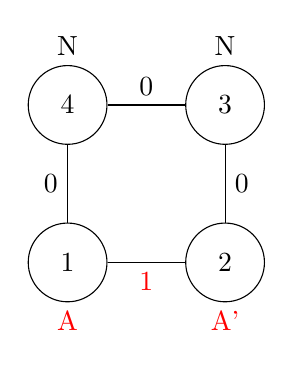
\begin{tikzpicture}
		\node[draw, circle, minimum size = 1 cm] (n1) at (0,0) {$1$};
		\node[draw, circle, minimum size = 1 cm] (n2) at (2,0) {$2$};
		\node[draw, circle, minimum size = 1 cm] (n3) at (2,2) {$3$};
		\node[draw, circle, minimum size = 1 cm] (n4) at (0,2) {$4$};
		
		\draw[-] (n1)--(n2)--(n3)--(n4);
		\draw[-] (n4)--(n1);
		
		\draw(0,-0.5) node[below] {\textcolor{red}{ A}};
		\draw(2,-0.5) node[below] {\textcolor{red}{A'}};
		\draw(2,2.5) node[above] {N};
		\draw(0,2.5) node[above] {N};
		
		\draw(1,0) node[below] {\textcolor{red}{1}};
		\draw(2,1) node[right] {0};
		\draw(1,2) node[above] {0};
		\draw(0,1) node[left] {0};
	\end{tikzpicture}
  %3 
  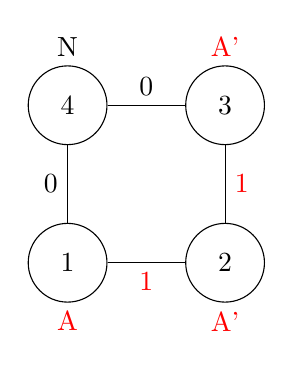
\begin{tikzpicture}
		\node[draw, circle, minimum size = 1 cm] (n1) at (0,0) {$1$};
		\node[draw, circle, minimum size = 1 cm] (n2) at (2,0) {$2$};
		\node[draw, circle, minimum size = 1 cm] (n3) at (2,2) {$3$};
		\node[draw, circle, minimum size = 1 cm] (n4) at (0,2) {$4$};
		
		\draw[-] (n1)--(n2)--(n3)--(n4);
		\draw[-] (n4)--(n1);
		
		\draw(0,-0.5) node[below] {\textcolor{red}{A}};
		\draw(2,-0.5) node[below] {\textcolor{red}{A'}};
		\draw(2,2.5) node[above] {\textcolor{red}{A'}};
		\draw(0,2.5) node[above] {N};
		
		\draw(1,0) node[below] {\textcolor{red}{1}};
		\draw(2,1) node[right] {\textcolor{red}{1}};
		\draw(1,2) node[above] {0};
		\draw(0,1) node[left] {0};
	\end{tikzpicture}

  %4 forbident r1 application 
  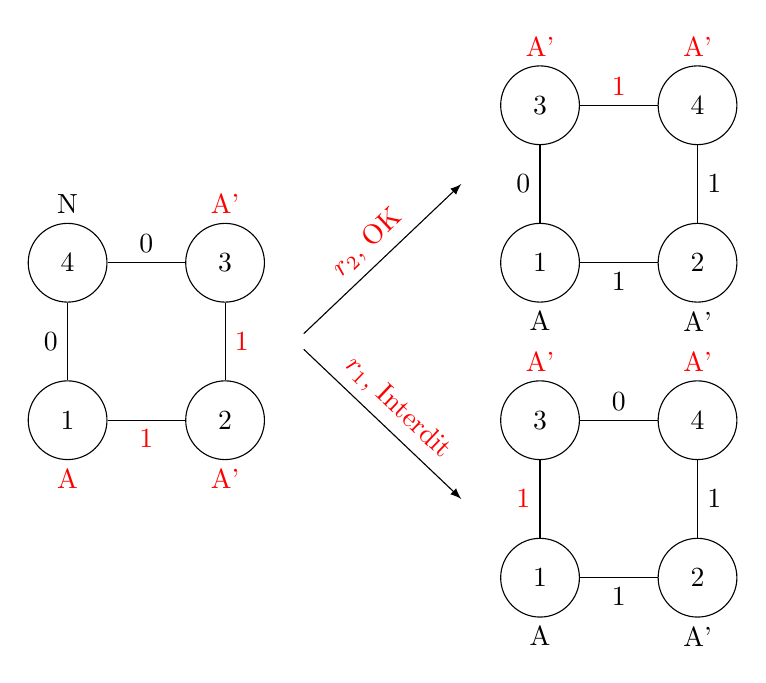
\begin{tikzpicture}
		\node[draw, circle, minimum size = 1 cm] (n1) at (0,0) {$1$};
		\node[draw, circle, minimum size = 1 cm] (n2) at (2,0) {$2$};
		\node[draw, circle, minimum size = 1 cm] (n3) at (2,2) {$3$};
		\node[draw, circle, minimum size = 1 cm] (n4) at (0,2) {$4$};
		
		\draw[-] (n1)--(n2)--(n3)--(n4);
		\draw[-] (n4)--(n1);
		
		\draw(0,-0.5) node[below] {\textcolor{red}{A}};
		\draw(2,-0.5) node[below] {\textcolor{red}{A'}};
		\draw(2,2.5) node[above] {\textcolor{red}{A'}};
		\draw(0,2.5) node[above] {N};
		
		\draw(1,0) node[below] {\textcolor{red}{1}};
		\draw(2,1) node[right] {\textcolor{red}{1}};
		\draw(1,2) node[above] {0};
		\draw(0,1) node[left] {0};


    %right up
	\node[draw, circle, minimum size = 1 cm] (2n1) at (6,2) {$1$};
	\draw (6,1.5) node[below]{A};
	\node[draw, circle, minimum size = 1 cm] (2n2) at (8,2) {$2$};
	\draw (8,1.5) node[below]{A'};
	\node[draw, circle, minimum size = 1 cm] (2n3) at (6,4) {$3$};
	\draw (6,4.5) node[above]{\textcolor{red}{A'}};
	\node[draw, circle, minimum size = 1 cm] (2n4) at (8,4) {$4$};
	\draw (8,4.5) node[above]{\textcolor{red}{A'}};


	\draw[-] (2n1)-- node[midway,below]{1}(2n2) -- node[midway,right]{1} (2n4) -- node[midway,above]{\textcolor{red}{1}} (2n3) --node[midway,left]{0} (2n1);
	
	
	%right down
	\node[draw, circle, minimum size = 1 cm] (2n1) at (6,-2) {$1$};
	\draw (6,-2.5) node[below]{A};
	\node[draw, circle, minimum size = 1 cm] (2n2) at (8,-2) {$2$};
	\draw (8,-2.5) node[below]{A'};
	\node[draw, circle, minimum size = 1 cm] (2n3) at (6,0) {$3$};
	\draw (6,0.5) node[above]{\textcolor{red}{A'}};
	\node[draw, circle, minimum size = 1 cm] (2n4) at (8,0) {$4$};
	\draw (8,0.5) node[above]{\textcolor{red}{A'}};
	
	
	\draw[-] (2n1)-- node[midway,below]{1}(2n2) -- node[midway,right]{1} (2n4) -- node[midway,above]{0} (2n3) --node[midway,left]{\textcolor{red}{1}} (2n1);
	
	\draw[->, >=latex] (3,1.1) to  node[sloped, midway,above]{\textcolor{red}{$r_2$, OK}} (5,3);
	\draw[->, >=latex] (3,0.9) to  node[sloped, midway,above]{\textcolor{red}{$r_1$, Interdit}} (5,-1);
\end{tikzpicture}
\end{example}